\documentclass[supercite]{Experimental_Report}

\title{~~~~~~新生实践课~~~~~~}
\author{陈永琪}
%\coauthor{张三、李四}
\school{计算机科学与技术学院}
\classnum{CS2309}
\stunum{U202315682}
%\costunum{U202115631、U202115631}
\instructor{陈加忠} % 该系列实验报告模板由华科大计院教师陈加忠制作
\date{2023年12月11日}

\usepackage{algorithm, multirow}
\usepackage{algpseudocode}
\usepackage{amsmath}
\usepackage{amsthm}
\usepackage{framed}
\usepackage{mathtools}
\usepackage{subcaption}
\usepackage{xltxtra} %提供了针对XeTeX的改进并且加入了XeTeX的LOGO, 自动调用xunicode宏包(提供Unicode字符宏)
\usepackage{bm}
\usepackage{tikz}
\usepackage{tikzscale}
\usepackage{pgfplots}
%\usepackage{enumerate}

\pgfplotsset{compat=1.16}

\newcommand{\cfig}[3]{
  \begin{figure}[htb]
    \centering
    \includegraphics[width=#2\textwidth]{images/#1.tikz}
    \caption{#3}
    \label{fig:#1}
  \end{figure}
}

\newcommand{\sfig}[3]{
  \begin{subfigure}[b]{#2\textwidth}
    \includegraphics[width=\textwidth]{images/#1.tikz}
    \caption{#3}
    \label{fig:#1}
  \end{subfigure}
}

\newcommand{\xfig}[3]{
  \begin{figure}[htb]
    \centering
    #3
    \caption{#2}
    \label{fig:#1}
  \end{figure}
}

\newcommand{\rfig}[1]{\autoref{fig:#1}}
\newcommand{\ralg}[1]{\autoref{alg:#1}}
\newcommand{\rthm}[1]{\autoref{thm:#1}}
\newcommand{\rlem}[1]{\autoref{lem:#1}}
\newcommand{\reqn}[1]{\autoref{eqn:#1}}
\newcommand{\rtbl}[1]{\autoref{tbl:#1}}

\algnewcommand\Null{\textsc{null }}
\algnewcommand\algorithmicinput{\textbf{Input:}}
\algnewcommand\Input{\item[\algorithmicinput]}
\algnewcommand\algorithmicoutput{\textbf{Output:}}
\algnewcommand\Output{\item[\algorithmicoutput]}
\algnewcommand\algorithmicbreak{\textbf{break}}
\algnewcommand\Break{\algorithmicbreak}
\algnewcommand\algorithmiccontinue{\textbf{continue}}
\algnewcommand\Continue{\algorithmiccontinue}
\algnewcommand{\LeftCom}[1]{\State $\triangleright$ #1}

\newtheorem{thm}{定理}[section]
\newtheorem{lem}{引理}[section]

\colorlet{shadecolor}{black!15}

\theoremstyle{definition}
\newtheorem{alg}{算法}[section]

\def\thmautorefname~#1\null{定理~#1~\null}
\def\lemautorefname~#1\null{引理~#1~\null}
\def\algautorefname~#1\null{算法~#1~\null}

\begin{document}

\maketitle

\clearpage

\pagenumbering{Roman}

\tableofcontents[level=2]

\clearpage

\pagenumbering{arabic}

\section{网页整体框架}

\begin{figure}[htb] % here top bottom
	\begin{center}
		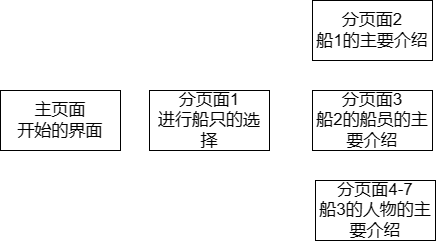
\includegraphics[scale=0.80]{images/drawio.png}
		\caption{网页整体框架}
		\label{fig1-1}
	\end{center}
\end{figure}
图1-1\ref{fig1-1}是我所设计的航海王主题网页的整体框架,包括一个主页面和七个分页面,主页提供开始按钮,分页面1提供三个船只选择,根据不同的选择可以跳转到不同的分页面,其中第一个选择对应分页面2,第二个选择对应分页面3,第三个选择对应分页面4-7,分页面4-7之间可以相互跳转,每个页面也都可以返回上一层。

\newpage

\section{主页设计}



\begin{figure}[htb]
	\begin{center}
		\includegraphics[scale=0.40]{images/zhu.png}
		\caption{主页}
		\label{fig2-1}
	\end{center}
\end{figure}

主页\textcolor{blue}{\ref{fig2-1}}的结构相对简单,将动漫中一个场景作为背景,背景中是航海王主角一团的主要人物,主要体现网页是以航海王为主题的,同时中间设置了一个航海王的标志性logo,并为其设置了一个超链接,可点击其跳转到分页面1,在页面的左上角也可点击返回寝室主页。


\newpage

\section{分页面设计}


\subsection{分页面1:船只选择}

\begin{figure}[htb]
	\begin{center}
		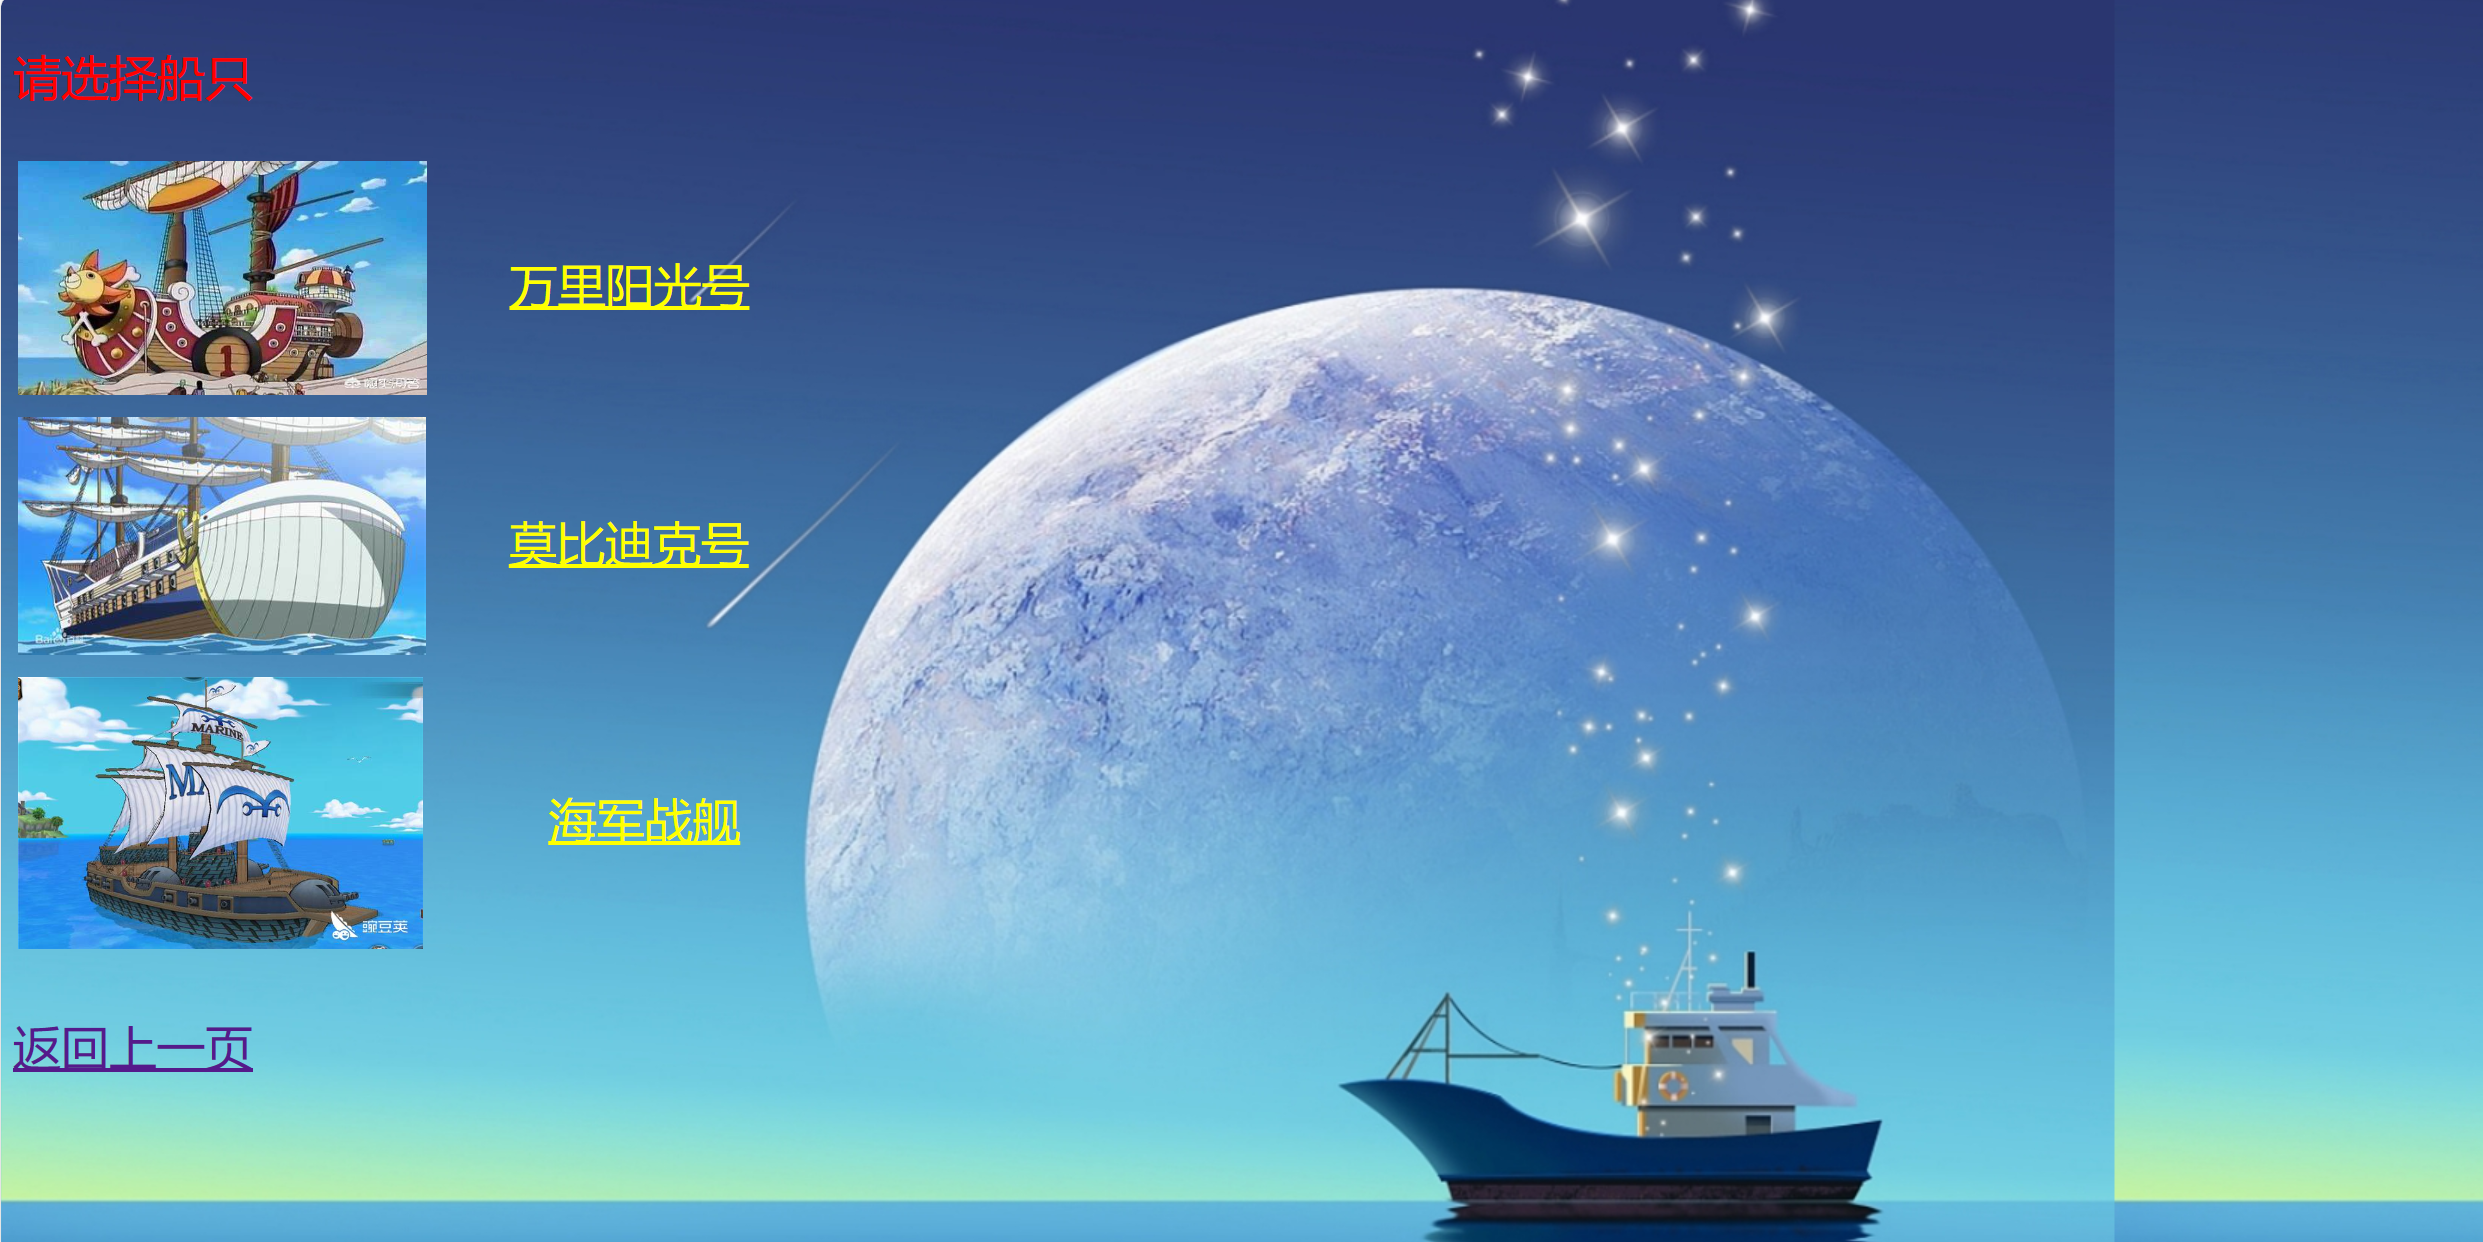
\includegraphics[scale=0.40]{images/fen1.png}
		\caption{船只选择}
		\label{fig3-1}
	\end{center}
\end{figure}

分页面1\textcolor{blue}{\ref{fig3-1}}主要提供三个船只的选择,分别提供了三只船的图片和名称,分别为万里阳光号、莫比迪克号和海军战舰,点击船只照片和船只名字均可跳转到该船只介绍的分页面,网页以一个船只作为背景,也体现了航海的元素,同时,左下角也提供了返回了主页面的链接。
\subsection{分页面2:万里阳光号}

\begin{figure}[htp]
	\begin{center}
		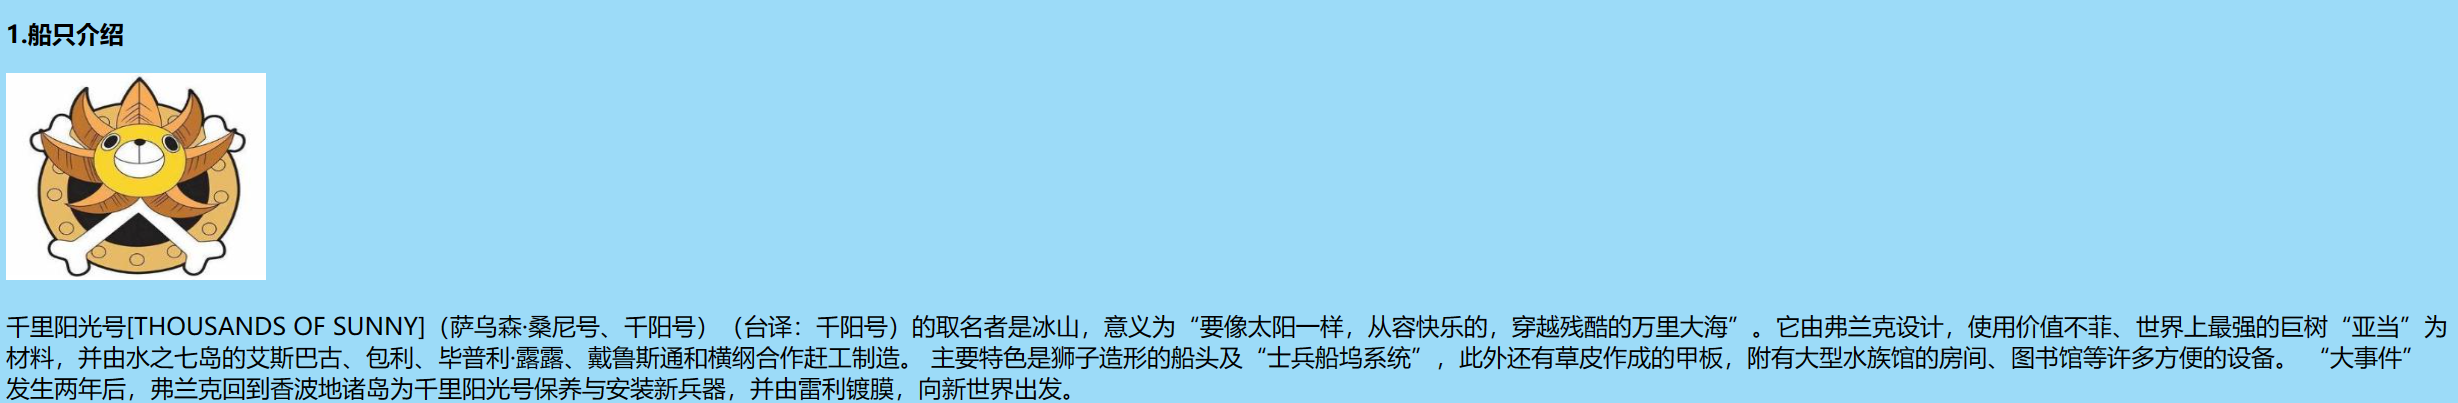
\includegraphics[scale=0.40]{images/fen2.2.png}
		\caption{万里阳光号-船只介绍}
		\label{fig3-2}
	\end{center}
\end{figure}
\newpage
\begin{figure}[htp]
	\begin{center}
		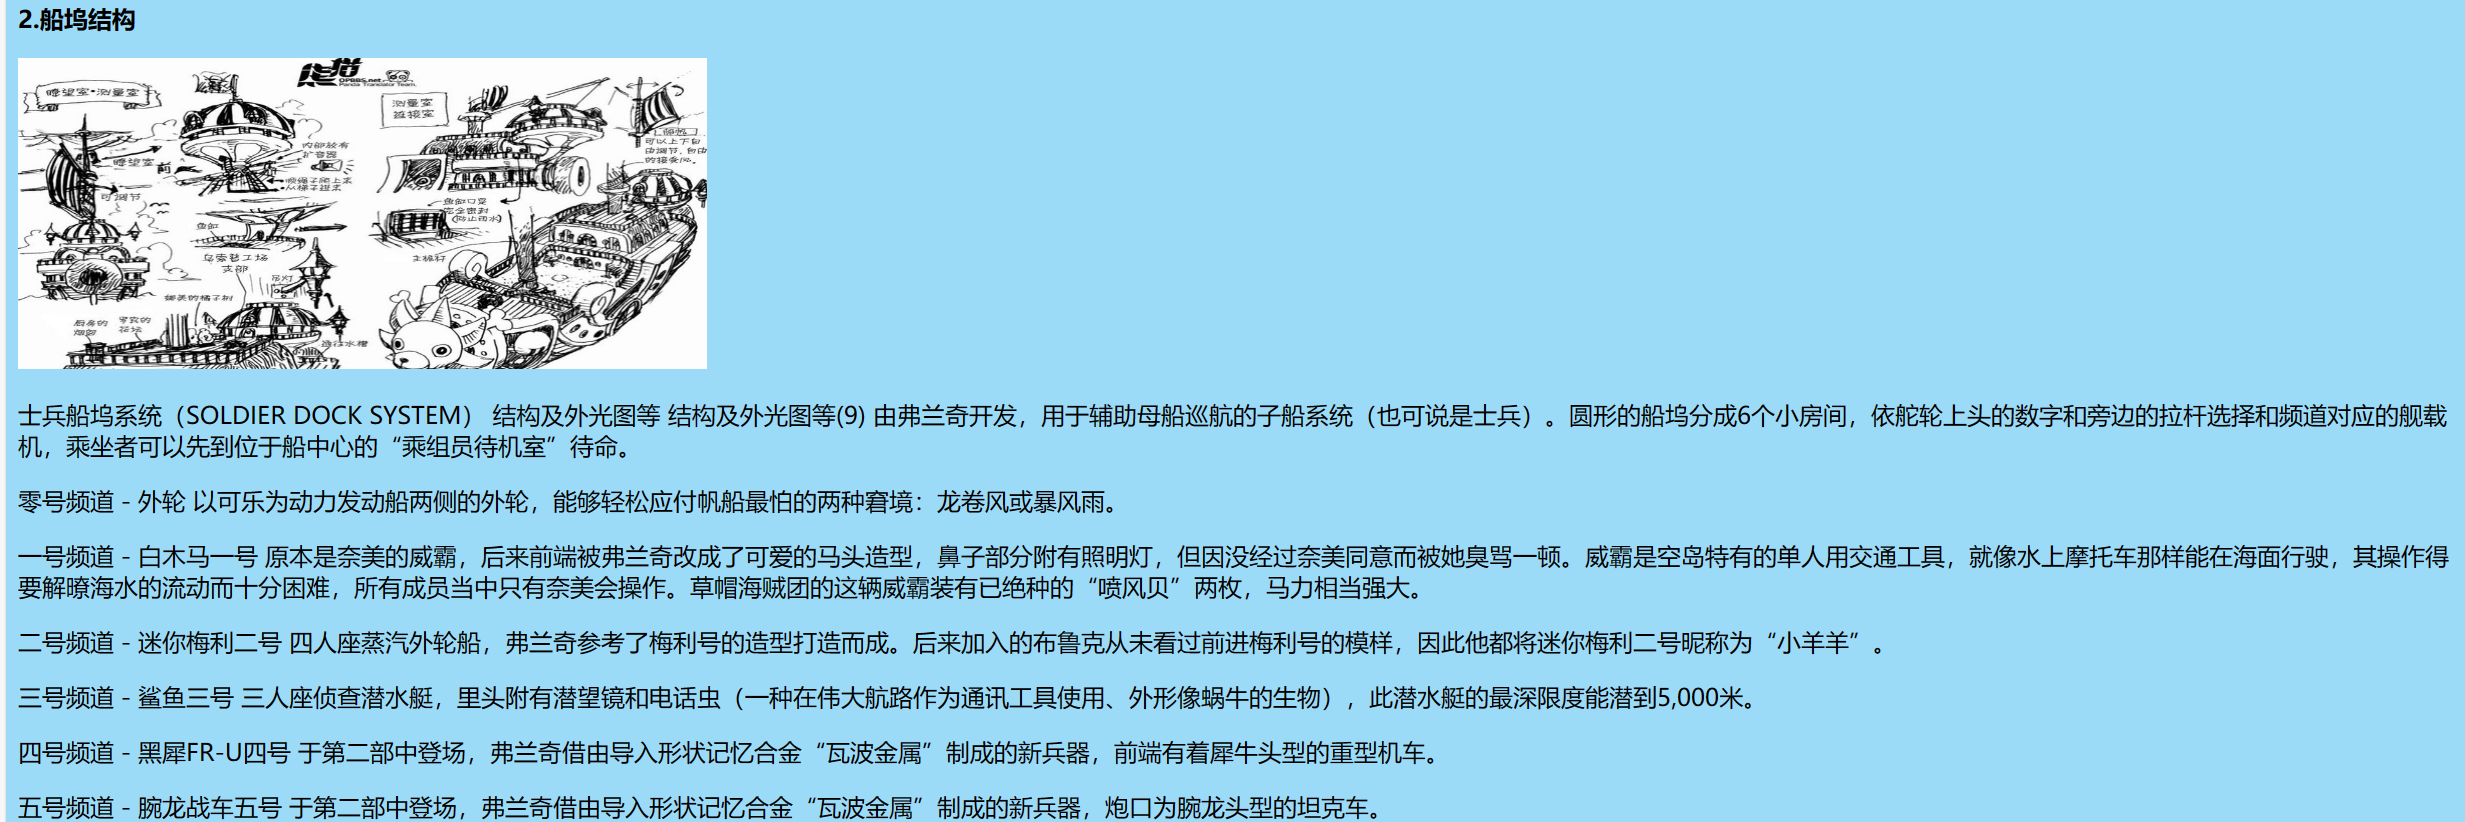
\includegraphics[scale=0.4]{images/fen2.3.png}
		\caption{万里阳光号-船坞结构}
		\label{fig3-3}
	\end{center}
\end{figure}
\begin{figure}[htp]
	\begin{center}
		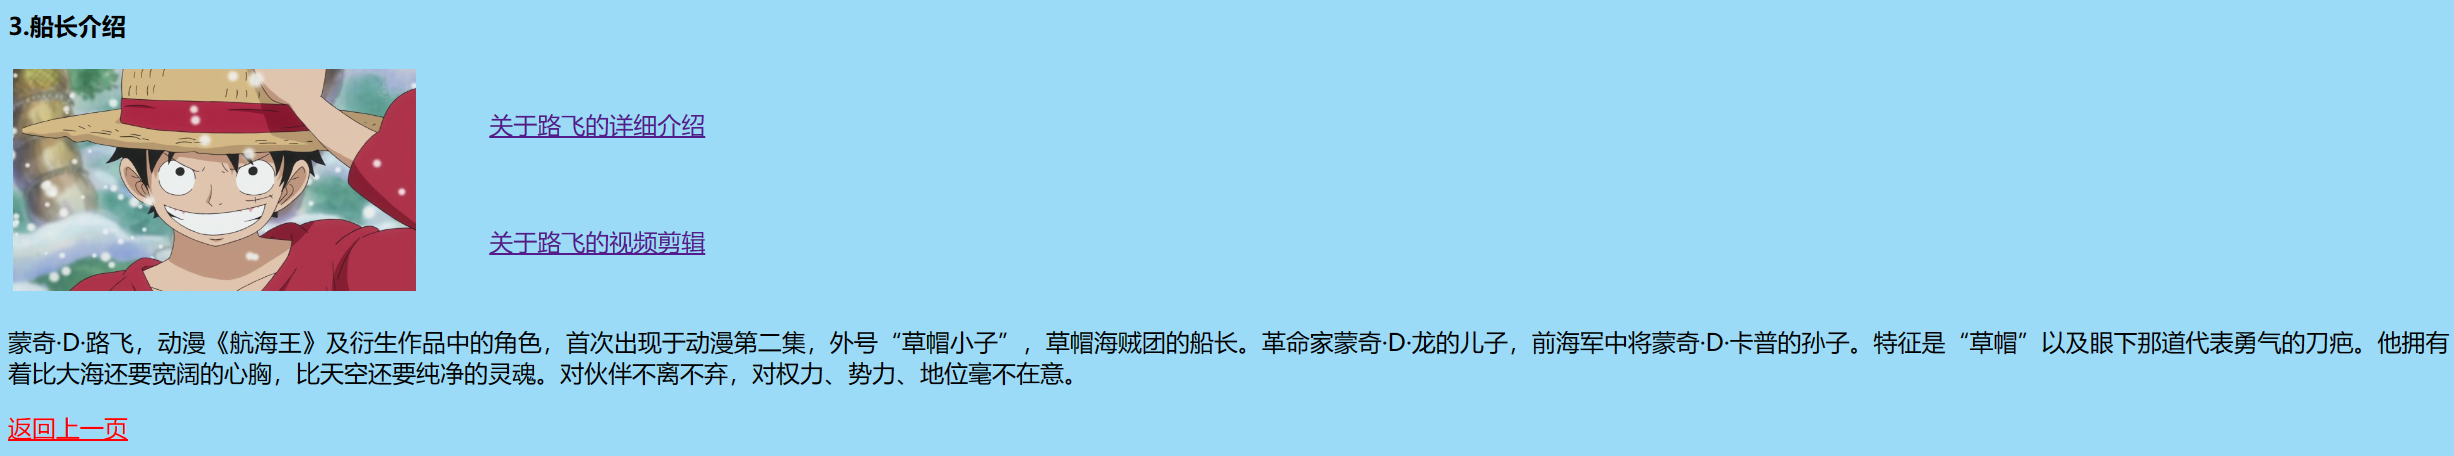
\includegraphics[scale=0.40]{images/fen2.1.png}
		\caption{万里阳光号-船长介绍}
		\label{fig3-4}
	\end{center}
\end{figure}
分页面2主要包含船只介绍\textcolor{blue}{\ref{fig3-2}}、船坞结构\textcolor{blue}{\ref{fig3-3}}和船长介绍\textcolor{blue}{\ref{fig3-4}}三个部分,其中每个部分都有图片和文字供观者对其形象和介绍进行了解,在船长介绍时,为了对主角路飞的信息进行补充,设置了两个外部链接,一个为其详细介绍,链接向百科,一个为其场面混剪,链接向视频网站,这两个链接都采用blank新建网页式,同时,最下方是返回按钮可返回分页面1。
\newpage
\subsection{分页面3:莫比迪克号}

\begin{figure}[htp]
	\begin{center}
		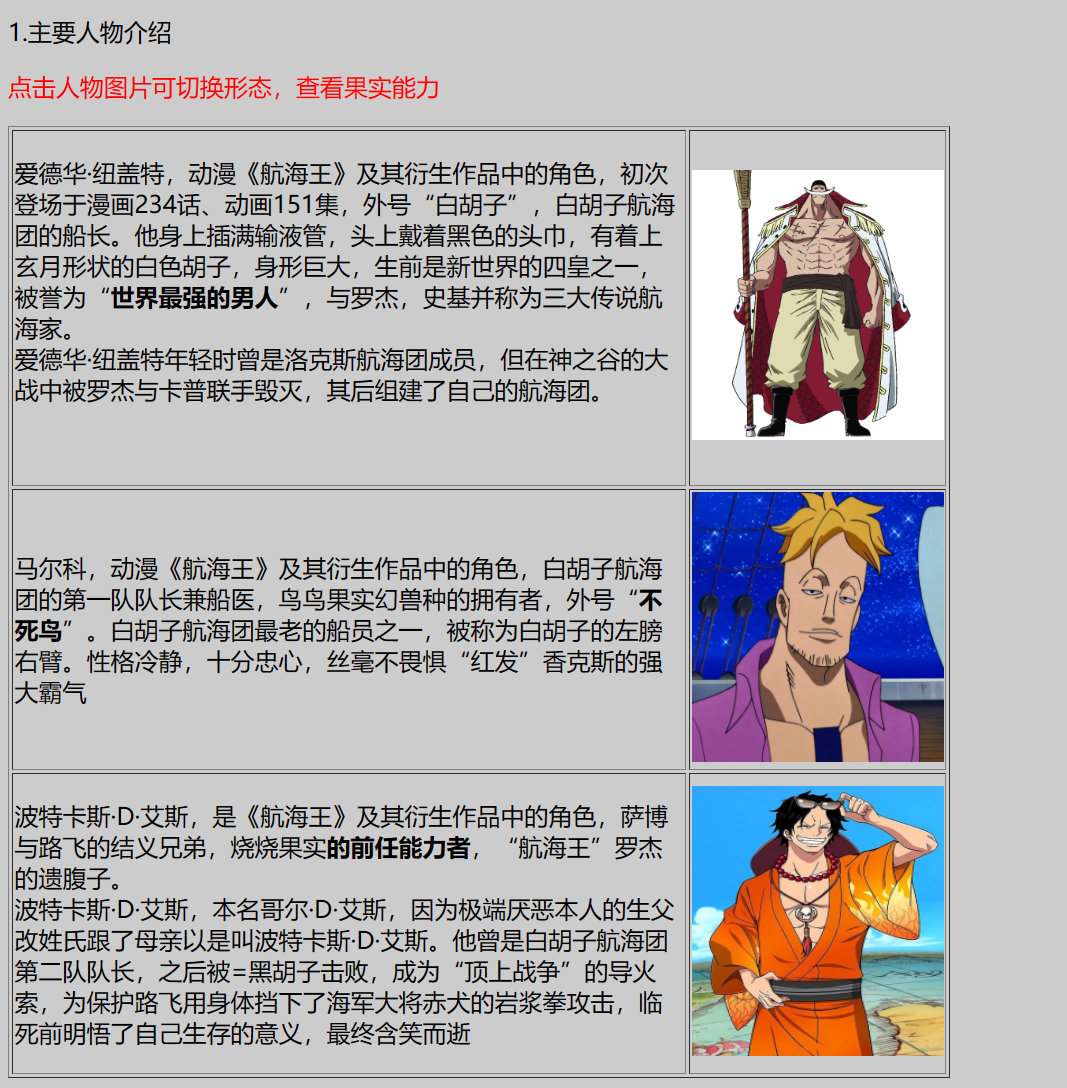
\includegraphics[scale=0.40]{images/fen3.1.png}
		\caption{莫比迪克号-主要人物}
		\label{fig3-5}
	\end{center}
\end{figure}
\begin{figure}[htp]
	\begin{center}
		
\includegraphics[scale=0.50]{images/fen3.2.png}
		\caption{莫比迪克号-主要介绍}
		\label{fig3-6}
	\end{center}
\end{figure}
\begin{figure}[htp]
	\begin{center}
		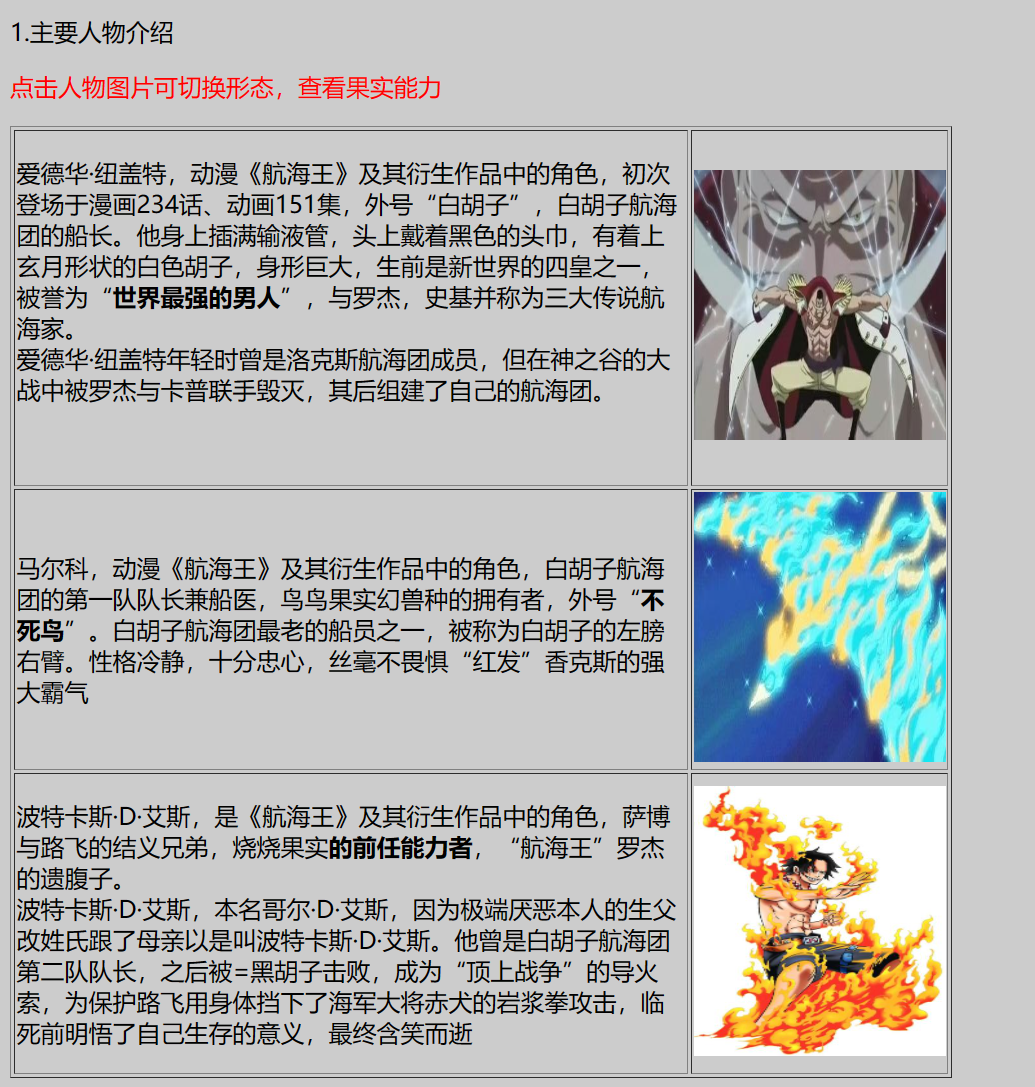
\includegraphics[scale=0.40]{images/fen3.3.png}
		\caption{莫比迪克号-主要人物2}
		\label{fig3-7}
	\end{center}
\end{figure}

分页面3主要包含主要人物介绍\textcolor{blue}{\ref{fig3-5}}和船只介绍\textcolor{blue}{\ref{fig3-6}},在主要人物介绍中,采用表格的方式对三个人物的身份经历进行了介绍,右边是其人物图像,点击图片后,图片会相应地进行改变,也如下一面所展示的\textcolor{blue}{\ref{fig3-7}}来让观者对人物的能力进行基本的了解,同时点击最下方返回上一页后,同样回返回分页面1。
\newpage
\subsection{分页面4-7:海军人物介绍}
以下是分页面4到7的其中一些图片,由于这几个页面是以有一定重复度的表格来展示的,故只展示几张典型图片。
\begin{figure}[htp]
	\begin{center}
		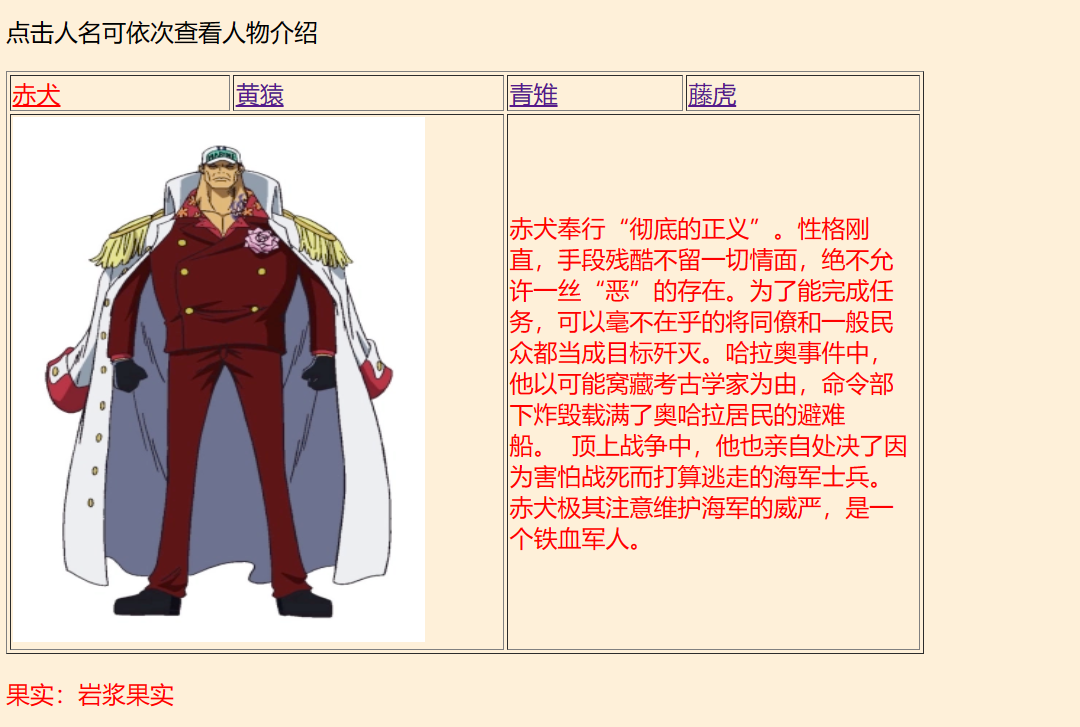
\includegraphics[scale=0.50]{images/fen4.1.png}
		\caption{赤犬-介绍}
		\label{fig3-8}
	\end{center}
\end{figure}
\begin{figure}[htp]
	\begin{center}
		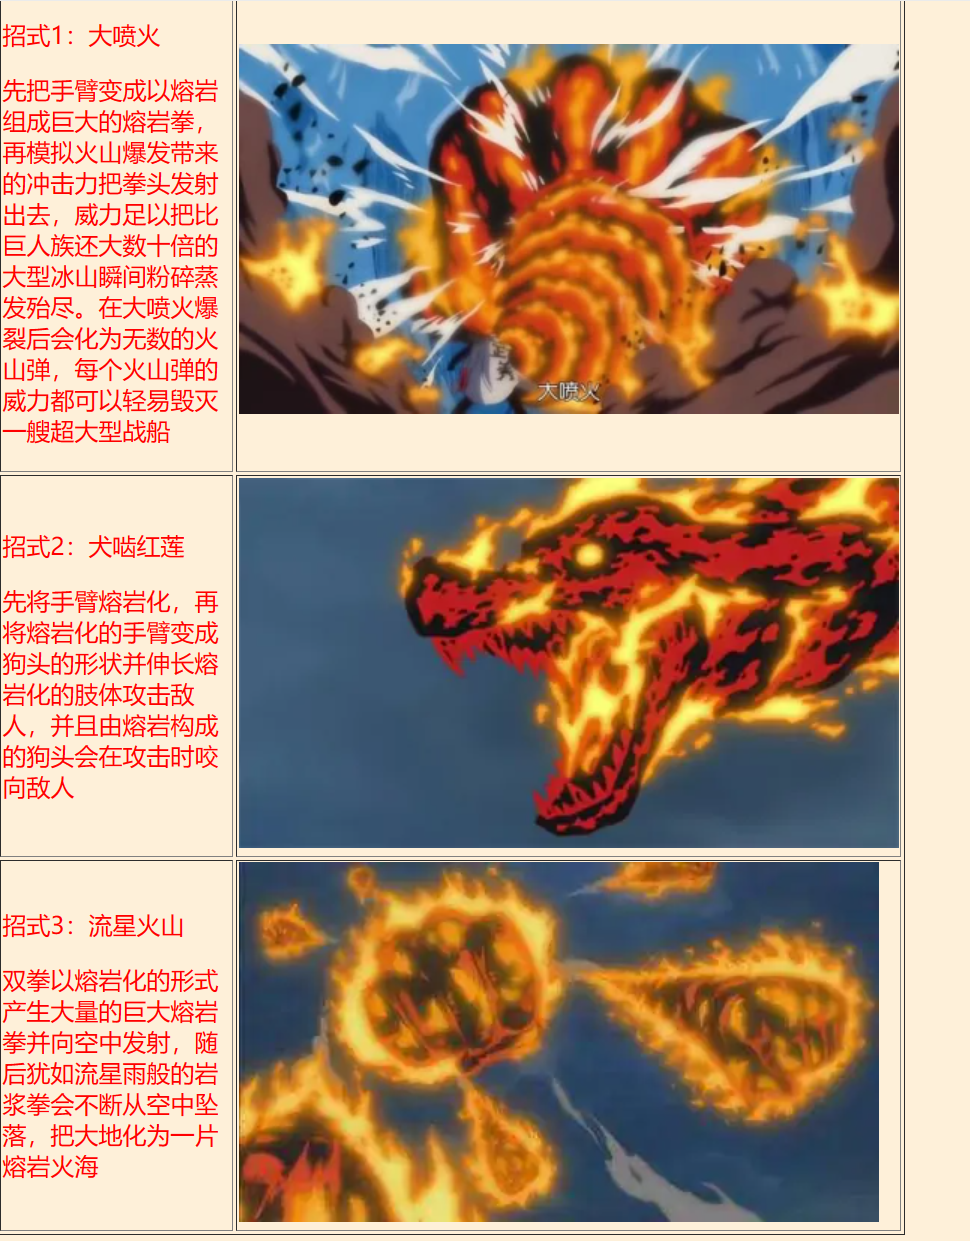
\includegraphics[scale=0.50]{images/fen4.2.png}
		\caption{赤犬-能力}
		\label{fig3-9}
	\end{center}
\end{figure}

\begin{figure}[htp]
	\begin{center}
		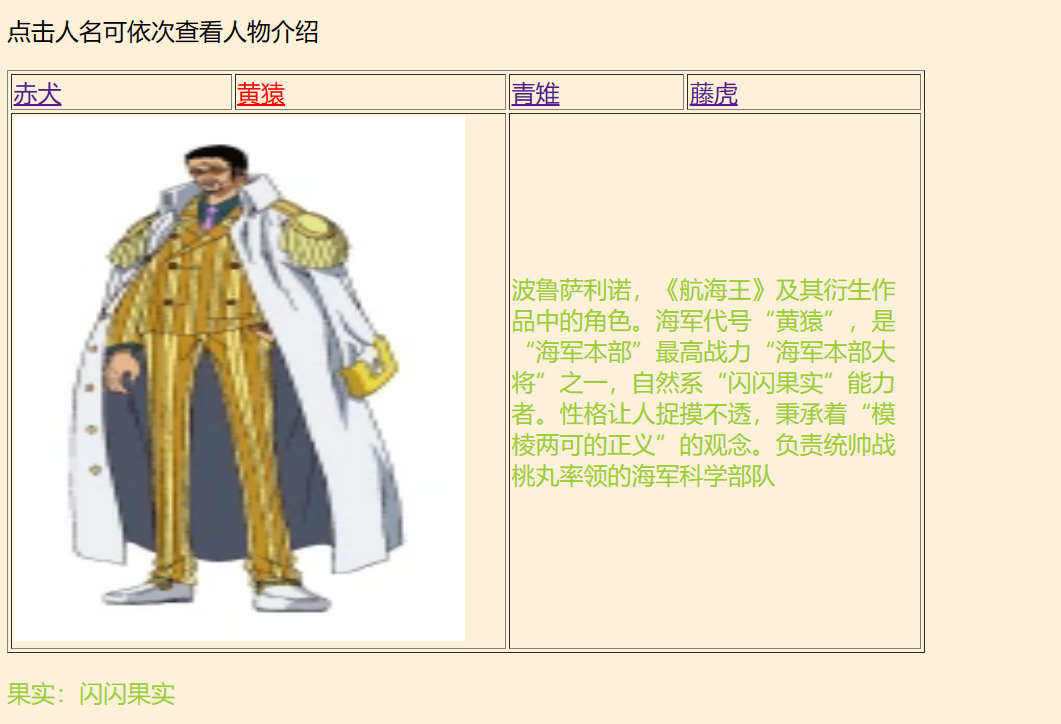
\includegraphics[scale=0.50]{images/fen5.1.png}
		\caption{黄猿-介绍}
		\label{fig3-10}
	\end{center}
\end{figure}
\newpage
\begin{figure}[htp]
	\begin{center}
		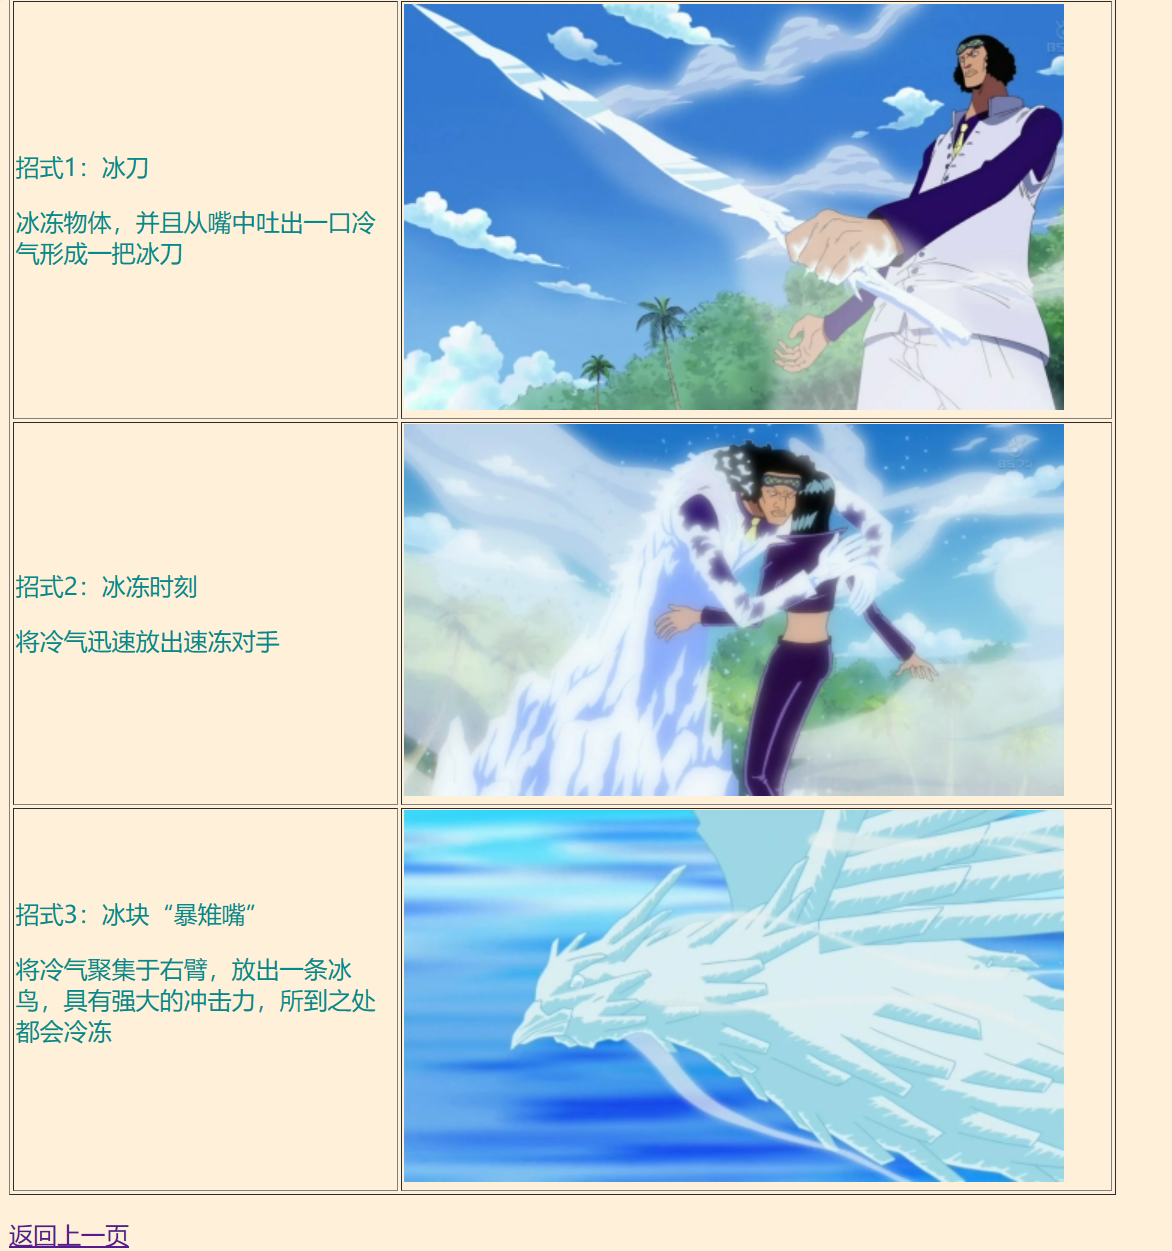
\includegraphics[scale=0.50]{images/fen6.2.png}
		\caption{青雉-能力}
		\label{fig3-11}
	\end{center}
\end{figure}

分页面4-7为一组页面,页面之间可以相互跳转,在每个页面点击返回上一页时返回的也都是分页面1,即船只选择所在的一个页面,4-7页面的上半部分为每个人物的身份和介绍,如\textcolor{blue}{\ref{fig3-8}},在选择其中人物时,该人物上方的名字会变为红色,表示现在所在页面,同时,在整个页面的文字颜色也根据人物的属性对颜色进行了调整,可对比\textcolor{blue}{\ref{fig3-8}}和\textcolor{blue}{\ref{fig3-10}},而每个页面的下半部分是对应角色的能力,同样是采用表格的方式呈现,左边为文字介绍,右边是能力对应的图片或者动图,如\textcolor{blue}{\ref{fig3-9}}和\textcolor{blue}{\ref{fig3-11}}.


\section{网页设计小结}

在网页的设计制作中,我遇到了许多问题,比如基础知识掌握不牢固,不会修改图片大小,使图片居中等,经过课件回顾和再次学习,对网页设计中一些类似最基本的操作也进行了巩固,但在设计背景时,又常常因为图片大小不合适而产生无法正确显示图片或者显示的图片作为背景不理想等状况,经过多次裁剪后,克服了这个问题。在设计分页面4到7时,又遇到了因为表格大小不合适而导致文字和图片变形等状况,经过查询和尝试,才终于解决。\par
可以说,本次学习与设计让我对网页是如何设计的有了更深的了解,在初步学习dw的基础知识和使用后,也对网页设计有了一些兴趣,在今后,我也希望能更加深入地了解html、css能的知识与操作,设计出交互性更强、观赏性更强的网页。


\newpage

\section{课程的收获和建议}


\subsection{计算机基础知识}

学习计算机基础知识,纯小白的我对资源管理器、安装路径、压缩软件等基础操作有了了解,对计算机专业所需电脑配置和不要装电脑管家这些内容有了认识,也提起了我进一步学习计算机的兴趣和热情。


\subsection{文档撰写工具LaTeX}

通过学习文档撰写工具LaTeX专题,我学会了如何使用命令行编译tex文件并生成pdf文件,也学会了LaTex中引用参考文献、插入图片、表示数学公式、添加切换颜色、为图片、公式等设置标签等基础知识,同时,也初步学会了如何建立表格、设置表格格式等内容。\par 但是,在初步学习时,也存在许多不足,如不太清楚如何为图片命名并进行引用跳转等,在逐渐学习后,才慢慢解决了这个问题,希望老师在今后讲授中也可以加强该块教学,让学生对LaTex掌握更加熟练。

\subsection{编程工具Python}

讲授Python时,可以着重强调Python中与C语言不同的部分,如要正确缩进、if等语句后边要加冒号等,同时着重讲述字典、元组、字符串、列表、集合等异同,如是否可以修改等,尤其对字典这个相对陌生的模型进行强调。\par
通过学习Python,我对其中一些基本元素和与C的区别有了基本的了解,也对如何定义函数、传递函数参数有初步的掌握,认识到了Python相对与C语言有许多便利的地方,如不需声明一个变量的类型,只需直接对其赋值,可在输入时采用input函数同时实现C中printf和scanf函数的输出输入作用等等。
\newpage

\subsection{图像设计软件Photoshop}

通过学习Visio,我对流程图中不同图形符号表示的不同意义有了掌握,如菱形框用于条件判断,平行四边形框用于输入输出等。\par
通过学习Photoshop,我学会了如何框选区域进取图片,如何混合图层,如何调整图片颜色,同时练习实践题后,我对如何对图片进行斜切,如何制作透明签名等也有了了解。\par
在Ps实践过程中,我也遇到许多问题,其中最突出的是不会将Ps后的图片做修改,导致导出后背景太大不利于操作,但在老师的指导下,我也学会了相应的操作,可以通过复制粘贴到新文件等操作才实现修改,在今后教学中,也希望老师加强这方面的教学。


\subsection{版本管理软件Git}

通过学习Git,我学会了如何在Gitee创建账号和远程仓库,如何克隆其他远程版本库到本地,如何通过命令行对文件进行推送,也在完成实践题的过程中学会了如何实现版本回退。\par
同时,上传文件到远程仓库是我觉得的一个容易出现问题的操作,我在实践过程中就因为搞错账号和昵称、未删除电脑上他人gitee账号而导致出错。


\subsection{网页制作Dreamweaver}

通过学习Dreamweaver,我了解了如何插入图像插入背景,如何更改背景文字链接等颜色,如何设置链接或增加外部链接,也了解了在设置链接步骤时self和blank的区别,尤其注意到了相对路径和绝对路径的区别。\par
在自己进行实践时,也简单学习了Dreamweaver的一些其他基础功能,如如何插入背景,如何设置按钮等操作,有很大的收获。




\end{document}